\documentclass[11pt]{article}

%==============Packages & Commands==============
\usepackage{graphicx}
\usepackage{fancyvrb}
\usepackage{tikz}
%%%<
\usepackage{verbatim}
%\usepackage[active,tightpage]{preview}
%\PreviewEnvironment{tikzpicture}
%\setlength\PreviewBorder{5pt}%

\usepackage{geometry}                		% See geometry.pdf to learn the layout options. There are lots.
% \geometry{a4paper}                   		% ... or a4paper or a5paper or ...
%\geometry{landscape}                		% Activat\usetikzlibrary{arrows}e for for rotated page geometry
%\usepackage[parfill]{parskip}    		% Activate to begin paragraphs with an empty line rather than an indent
\usepackage{graphicx}				% Use pdf, png, jpg, or eps§ with pdflatex; use eps in DVI mode
								% TeX will automatically convert eps --> pdf in pdflatex
\usepackage{amssymb}

\usepackage[ruled,vlined]{algorithm2e}
\usetikzlibrary{arrows}
\usepackage{alltt}
\usepackage[T1]{fontenc}
\usepackage[utf8]{inputenc}
\usepackage{indentfirst}
\usepackage[longnamesfirst]{natbib} % For references
\bibpunct{(}{)}{;}{a}{}{,} % Reference punctuation
\usepackage{changepage}
\usepackage{setspace}
\usepackage{booktabs} % For tables
\usepackage{rotating} % For sideways tables/figures
\usepackage{amsmath}
\usepackage{multirow}
\usepackage{color}
\usepackage{dcolumn}
\usepackage{comment}
%\usepackage{fullwidth}
\newcolumntype{d}[1]{D{.}{\cdot}{#1}}
\newcolumntype{.}{D{.}{.}{-1}}
\newcolumntype{3}{D{.}{.}{3}}
\newcolumntype{4}{D{.}{.}{4}}
\newcolumntype{5}{D{.}{.}{5}}
\usepackage{float}
\usepackage[hyphens]{url}
%\usepackage[margin = 1.25in]{geometry}
%\usepackage[nolists,figuresfirst]{endfloat} % Figures and tables at the end
\usepackage{subfig}
\captionsetup[subfloat]{position = top, font = normalsize} % For sub-figure captions
\usepackage{fancyhdr}
%\makeatletter
%\def\url@leostyle{%
%  \@ifundefined{selectfont}{\def\UrlFont{\sf}}{\def\UrlFont{\small\ttfamily}}}
%\makeatother
%% Now actually use the newly defined style.
\urlstyle{same}
\usepackage{times}
% \usepackage{mathptmx}
%\usepackage[colorlinks = true,
%						bookmarksopen = true,
%						pagebackref = true,
%						linkcolor = black,
%						citecolor = black,
% 					urlcolor = black]{hyperref}
%\usepackage[all]{hypcap}
%\urlstyle{same}
\newcommand{\fnote}[1]{\footnote{\normalsize{#1}}} % 12 pt, double spaced footnotes
\def\citeapos#1{\citeauthor{#1}'s (\citeyear{#1})}
\def\citeaposs#1{\citeauthor{#1}' (\citeyear{#1})}
\newcommand{\bm}[1]{\boldsymbol{#1}} %makes bold math symbols easier
\newcommand{\R}{\textsf{R}\space} %R in textsf font
\newcommand{\netinf}{\texttt{NetInf}\space} %R in textsf font
\newcommand{\iid}{i.i.d} %shorthand for iid
\newcommand{\cites}{{\bf \textcolor{red}{CITES}}} %shorthand for iid
%\usepackage[compact]{titlesec}
%\titlespacing{\section}{0pt}{*0}{*0}
%\titlespacing{\subsection}{0pt}{*0}{*0}
%\titlespacing{\subsubsection}{0pt}{*0}{*0}
%\setlength{\parskip}{0pt}
%\setlength{\parsep}{0pt}
%\setlength{\bibsep}{2pt}
%\renewcommand{\headrulewidth}{0pt}

%\renewcommand{\figureplace}{ % This places [Insert Table X here] and [Insert Figure Y here] in the text
%\begin{center}
%[Insert \figurename~\thepostfig\ here]
%\end{center}}
%\renewcommand{\tableplace}{%
%\begin{center}
%[Insert \tablename~\theposttbl\ here]
%\end{center}}

\newcommand\independent{\protect\mathpalette{\protect\independenT}{\perp}}
\def\independenT#1#2{\mathrel{\rlap{$#1#2$}\mkern2mu{#1#2}}}
\newcommand{\N}{\mathcal{N}}
\newcommand{\Y}{\bm{\mathcal{Y}}}
\newcommand{\bZ}{\bm{Z}}

\usepackage[colorlinks = TRUE, urlcolor = black, linkcolor = black, citecolor = black, pdfstartview = FitV]{hyperref}


%============Article Title, Authors==================
\title{\vspace{-2cm} Content of Municipal Government Websites }


\author{ Markus Neumann \and Bruce Desmarais \and Hanna Wallach} \date{\today}



%===================Startup=======================
\begin{document}
\maketitle



%=============Abstract & Keywords==================

\begin{abstract}

\noindent We study the content of municipal government websites....

\end{abstract}
\thispagestyle{empty}
% \doublespacing
% Description of the possible challenges
\section{Introduction}

\section{Data}
The General Services Administration (GSA) maintains all .gov addresses, and provides a complete\footnote{Domains used for testing and internal programs are excluded.} list of all such domains to the public through GitHub\footnote{https://github.com/GSA/data/tree/gh-pages/dotgov-domains}. This list is updated once per month - we rely on the version released on January 16, 2017. The data from the GSA contains the following variables: One, domain name, specifically, the all-uppercase version of domain and top-level domain (for example, 'ABERDEENMD.GOV'). Two, the type of government entity to which the domain is registered, such as city, county, federal agency, etc. Three, for federal agencies, the name is specfied. Finally, the city in which the domain is registered, is noted.

Here, we focus only on cities. As a first step, we use a webdriver-controlled browser (Firefox/Selenium/Geckodriver) to test whether all of the city websites actually work. Of the 2425 domains listed by the GSA as cities, 292 are not accessible. Furthermore, the .gov domain, as registered at the GSA, is frequently not the website a city actually uses. In many cases, these sites redirect to another address, sometimes not a .gov domain (in this case, we simply use this domain). We record these URLs, as they are required to retrieve the images websites stored in the Wayback Machine (WbM).

In order to provide an overview of our coverage (as not all cities, towns and villages use .gov addresses), we merge this list with U.S. Census data\footnote{http://www2.census.gov/programs-surveys/popest/datasets/2010-2015/cities/totals/sub-est2015\_all.csv}. Here, several limitations in the GSA data need to be accounted for: One, even though the GSA nominally separates websites of cities and counties, some of the domains categorized as cities actually belong to counties. The same is true for townships and boroughs. Ergo, we eliminate all websites belonging to these three types of entities by hand. Furthermore, the city name, as given by the GSA, refers to the city in which the domain is registered, which is not necessarily equivalent to the city the website serves. In many cases, a website of a larger city may be registered to one of its subdivisions (for example, the website of New York is registered to Brooklyn), or vice versa (for example, the website of Homecroftin, a small town within Indianapolis, is registered to the city as a whole). Consequently we fix mismatches between websites and cities manually. Finally, a number of cities are simply misspelled, which we also correct by hand.

After the counties, townships and cities that cannot be matched to the Census data\footnote{There are five cities that are not contained in the Census data} and duplicate websites (some cities have more than one website) are removed, 1813 domains/cities remain.

These cities contain 90,616,865 people, and thus about 28\% of the U.S. population (see figure 1).

\begin{figure}[!ht]
	\centering
	%\caption{Population coverage}
	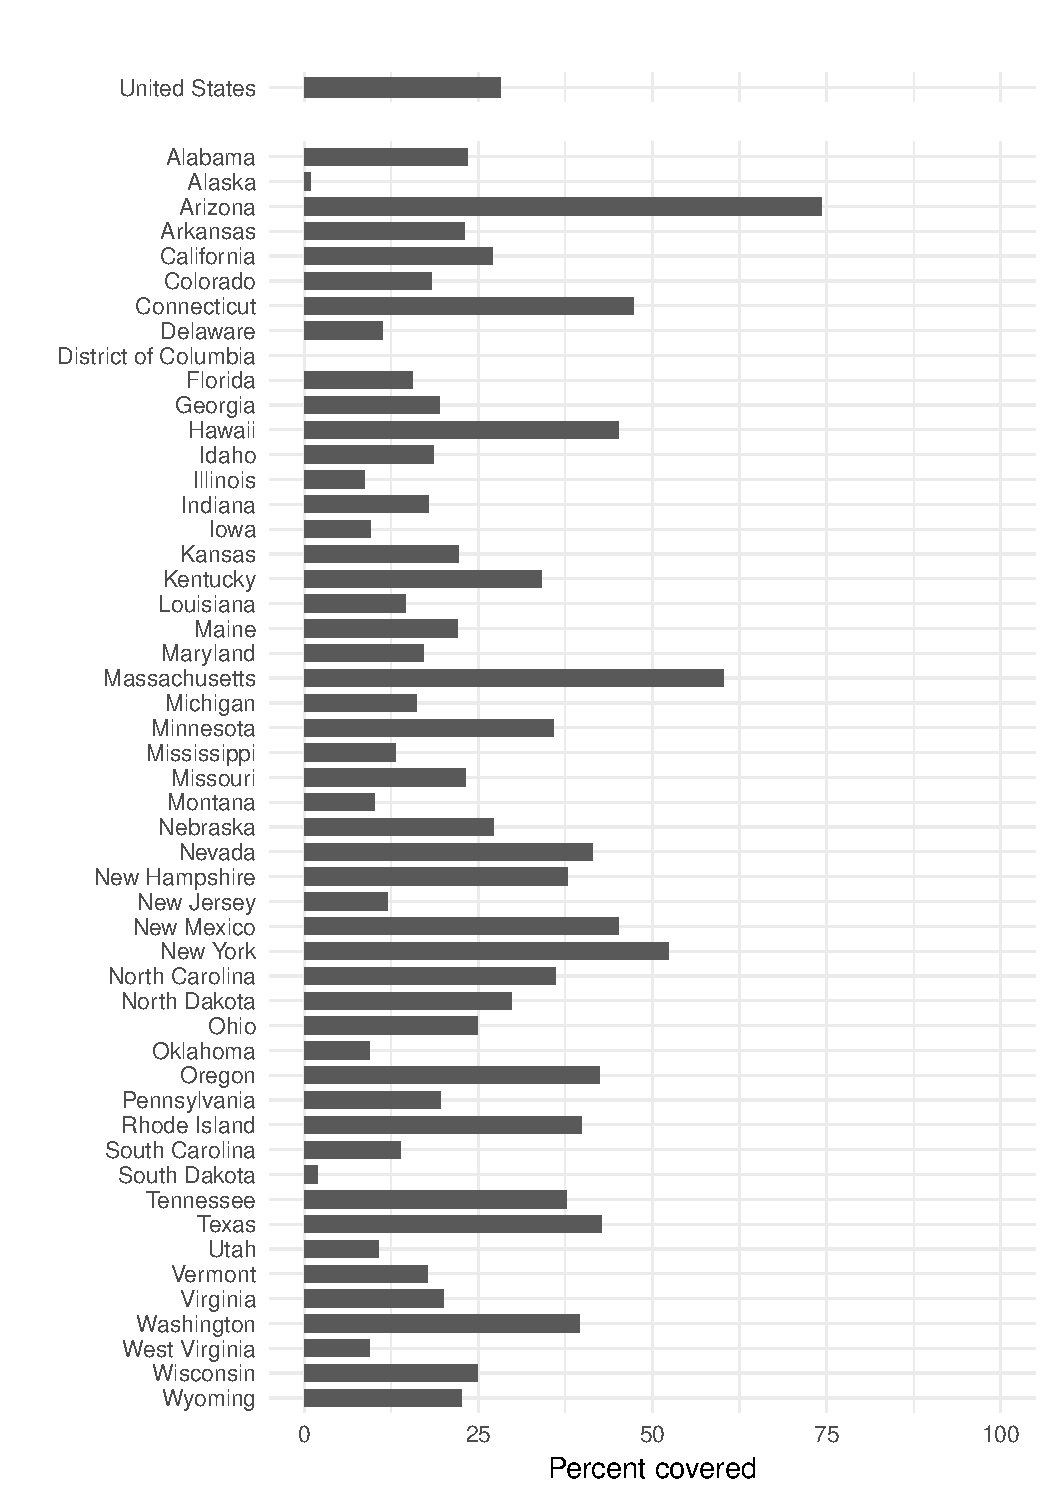
\includegraphics[width=0.9\linewidth,height=0.9\textheight]{figures/coverage_states.pdf}
\end{figure}

We use the resulting list of websites to acccess their copies stored in the Internet Archive's Wayback Machine. To this end, we rely on the Ruby Gem 'Wayback Machine Downloader'\footnote{https://github.com/hartator/wayback-machine-downloader} (WbMD). We supply the URL that each .gov website redirects to to the WbMD, which then downloads every file present in the WbM from a snapshot in October 2016, or, if not available, as soon as possible after this point.

<Note: We have not actually done this last step for all websites (however, the R script which runs the Ruby package is already set up to do so once we need to). Instead 10 websites were randomly sampled from an older version of the GSA list, which still contained counties and townships, which is why one of the 10 websites is from Dutchess County, NY.>

% latex table generated in R 3.3.2 by xtable 1.8-2 package
% Wed Feb 22 21:39:50 2017
\begin{table}[ht]
	\centering
	\begin{tabular}{lr}
		\hline
		File type & Occurrences \\ 
		\hline
		.pdf & 1371 \\ 
		.html & 819 \\ 
		.png & 210 \\ 
		.jpg & 131 \\ 
		.gif &  99 \\ 
		.js &  51 \\ 
		.PDF &  50 \\ 
		.aspx &  43 \\ 
		.doc &  35 \\ 
		.css &  32 \\ 
		.JPG &  26 \\ 
		.Net &  12 \\ 
		.xlsx &   6 \\ 
		.docx &   5 \\ 
		.ttf &   3 \\ 
		.xml &   3 \\ 
		.htm &   2 \\ 
		.woff &   2 \\ 
		.xls &   2 \\ 
		.asp &   1 \\ 
		.eot &   1 \\ 
		.GIF &   1 \\ 
		.ico &   1 \\ 
		.PNG &   1 \\ 
		.ppt &   1 \\ 
		.swf &   1 \\ 
		.txt &   1 \\ 
		\hline
	\end{tabular}
	\caption{File types in scraped websites} 
\end{table}

% latex table generated in R 3.3.2 by xtable 1.8-2 package
% Wed Feb 22 21:35:10 2017
\begin{table}[ht]
	\centering
	\begin{tabular}{lrr}
		\hline
		Website & Files & Size (MB) \\ 
		\hline
		brownsvilletn.gov & 188 & 14328 \\ 
		www.centralpointoregon.gov & 150 & 137440 \\ 
		www.dedham-ma.gov & 603 & 212572 \\ 
		www.duncanok.gov &  84 & 47064 \\ 
		www.dutchessny.gov & 110 & 291376 \\ 
		www.ennistx.gov & 200 & 26244 \\ 
		www.greenvillenc.gov & 333 & 25732 \\ 
		www.romi.gov & 491 & 112584 \\ 
		www.trumbull-ct.gov & 787 & 191540 \\ 
		www.westonct.gov & 861 & 213140 \\ 
		\hline
	\end{tabular}
	\caption{Test websites} 
\end{table}

\newpage

\bibliographystyle{apsr}
\bibliography{ref}

\end{document}
